\documentclass[11pt,a4paper]{article}
\usepackage[T1]{fontenc}
\usepackage[margin=2.3cm]{geometry}
\usepackage{amsmath,amssymb}
\usepackage{graphicx}
\usepackage[dvipsnames]{xcolor}
\usepackage{enumitem}
\usepackage[colorlinks=true,linkcolor=blue,urlcolor=blue]{hyperref}
\setlength{\parskip}{0.6em}
\setlength{\parindent}{0pt}
\begin{document}

\begin{center}{\LARGE\bfseries openheatspread}\\[0.4em]{\large Predict where a laptop gets hot, in three sessions.}\\[0.2em]\small PAN IIT OSS explainer \textbullet{} higher secondary to diploma / undergraduate (levels 4-5)\end{center}

\section*{Why this exists}
Every electronic device turns some of its power into heat that has to leave through a path of solids and air. This explainer shows the mathematics of that heat flow, from one slab to a 2D simulation, using only elementary physics and arithmetic, so you can build it yourself.

\section*{The end goal}
Predict laptop hot spots with heat diffusion. The end goal is to predict where a laptop gets hot: finding hot spots with heat diffusion. The same mathematics governs cooling of batteries, buildings, engine parts and food.

\section*{How the three sessions build up}
\begin{enumerate}[nosep]
\item \textbf{Session 1: Heat flows through a slab: Fourier's law} (Level 1, conceptual interactive model, 60 min).
\item \textbf{Session 2: Thermal resistance: layers in series and a cooling design} (Level 2, mathematical engineering model, 75 min).
\item \textbf{Session 3: A 2D heat solver, validated, and a laptop with two hot spots} (Level 3, simulation and validation, 90 min).
\end{enumerate}

\section{Session 1: Heat flows through a slab: Fourier's law}

\subsection*{A. Real-world problem}
The chip inside a laptop turns electricity into heat. The heat must get out through a thin pad into a metal heatsink, and the chip is safe only while it stays cool enough. How fast does heat move through a layer, how does the temperature change as you go through it, and why does a thin copper plate carry so much more heat than a slab of glass of the same size? This is general education about heat flow, not a design method for real products.

\subsection*{B. Concept and theory}
Heat is energy moving because of a temperature difference; it always flows from the hotter side to the colder side. In steady state (nothing changing with time) the heat flow through a flat slab is proportional to the area A, to the temperature difference between its faces, and to the material's thermal conductivity k, and inversely proportional to the thickness L. Because the same heat must cross every layer of the slab, the temperature falls at a constant rate, so the profile is a straight line from the hot face to the cold face. The line does not depend on k; k only decides how much heat the slab carries.

\begin{itemize}[nosep]
\item Q: heat flow (heat per second) (W)
\item k: thermal conductivity of the material (W/(m K))
\item A: area the heat passes through (1 cm\textasciicircum{}2 = 0.0001 m\textasciicircum{}2) (m\textasciicircum{}2)
\item T\_hot, T\_cold: temperatures of the two faces (C)
\item L: slab thickness (heat travel distance) (m)
\item q: heat flux, heat flow per unit area (W/m\textasciicircum{}2)
\item R: thermal resistance of the slab (K/W)
\end{itemize}

\begin{equation*}
Q=\frac{k\,A\,(T_{hot}-T_{cold})}{L}
\end{equation*}

\begin{equation*}
T(x)=T_{hot}-\left(T_{hot}-T_{cold}\right)\frac{x}{L},\qquad 0\le x\le L
\end{equation*}

\begin{equation*}
q=\frac{Q}{A}=\frac{k\,(T_{hot}-T_{cold})}{L},\qquad R=\frac{L}{kA}
\end{equation*}

\begin{center}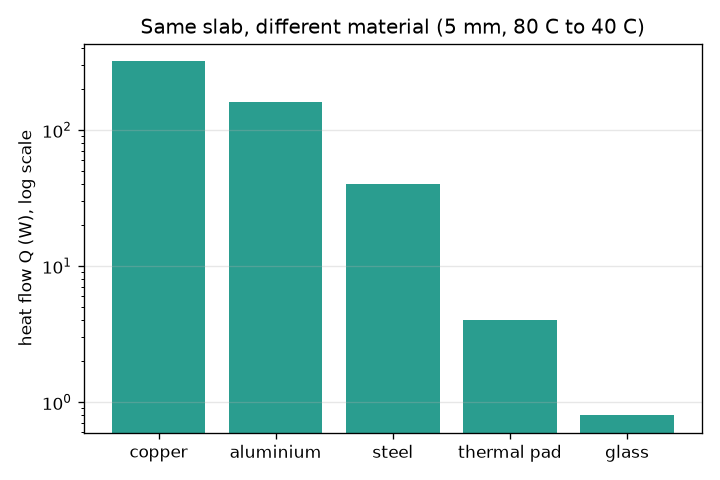
\includegraphics[width=0.85\linewidth]{figures/s01_heat_by_material.png}\\\small Heat flow through the same slab in five materials (log scale): conductivity sets how much heat flows.\end{center}

\subsection*{E. Worked example}
A thermal pad (k = 5 W/(m K)) is 1 mm thick and covers 1 cm\textasciicircum{}2. Its hot face is at 80 C and its cold face at 50 C. Find the heat flow, the heat flux and the temperature half way through.
\begin{enumerate}[nosep]
\item Convert to metres: L = 1 mm = 0.001 m, A = 1 cm\textasciicircum{}2 = 0.0001 m\textasciicircum{}2.
\item Q = k A (T\_hot - T\_cold) / L = 5 * 0.0001 * 30 / 0.001 = 15 W.
\item Flux q = Q / A = 15 / 0.0001 = 150000 W/m\textasciicircum{}2.
\item The profile is a straight line, so half way (x = 0.5 mm) the temperature is the average: (80 + 50) / 2 = 65 C.
\item Sanity check: 15 W is a reasonable laptop-chip power, and a 30 C drop across a pad this thin is what real pads show.
\end{enumerate}
\textbf{Answer.} Q = 15 W, q = 150000 W/m\textasciicircum{}2 and the middle of the pad is at 65 C.

\subsection*{F. Questions}
\begin{enumerate}[nosep]
\item \textbf{Conceptual.} A slab of copper and a slab of glass have the same size and the same face temperatures. Which has the larger temperature drop per millimetre, and which carries more heat? Explain.
\item \textbf{Numerical.} A thermal pad with k = 5 W/(m K) is 0.5 mm thick and covers 1 cm\textasciicircum{}2, with faces at 70 C and 50 C. Find the heat flow in W and check that the answer is sensible.
\item \textbf{Graph and simulation interpretation.} In the profile graph for L = 2, 5 and 10 mm (80 C to 40 C), what is the temperature at a depth of 2 mm in each slab, and what does that tell you about the slope?
\item \textbf{Design and optimisation challenge.} Design: a pad (k = 5 W/(m K), 1 cm\textasciicircum{}2) must carry at least 12 W from a chip face at 80 C to a heatsink face at 50 C. Manufacturing says it cannot be thinner than 0.3 mm. Choose a thickness and justify it.
\end{enumerate}

\section{Session 2: Thermal resistance: layers in series and a cooling design}

\subsection*{A. Real-world problem}
A laptop chip dissipates 20 W. Its heat crosses a smear of thermal paste, an aluminium heatsink base and finally the air blown across the fins by a fan. The chip must stay below 85 C when the room is 25 C. If it runs too hot, what do you change: use copper instead of aluminium, make the base thicker, or spin the fan faster? Which one actually helps? This is a simplified model for learning, not a validated cooling design.

\subsection*{B. Concept and theory}
Rearranging Fourier's law gives dT = Q R, which looks like Ohm's law with temperature difference as voltage and heat flow as current. A conducting layer has R = L/(kA). Heat carried away by moving air obeys Newton's law of cooling, Q = h A dT, so the film of air has R = 1/(hA). When the same heat Q = P passes through layers one after another, the resistances add. The chip (junction) temperature is the ambient temperature plus P times the total resistance, and the temperature drop across each layer is P times that layer's resistance.

\begin{itemize}[nosep]
\item P: chip power (all of it becomes heat) (W)
\item T\_amb: air temperature (25 C) (C)
\item R\_paste, R\_base, R\_air: thermal resistances of paste, base and the air film (K/W)
\item h: convection coefficient: how well moving air carries heat off a surface (W/(m\textasciicircum{}2 K))
\item A\_base: base area (20 mm x 20 mm = 4 cm\textasciicircum{}2) (m\textasciicircum{}2)
\item A\_fins: total fin surface touched by air (100 cm\textasciicircum{}2, assumed) (m\textasciicircum{}2)
\item L, k: base thickness and conductivity (m, W/(m K))
\item T\_chip: chip temperature (C)
\end{itemize}

\begin{equation*}
R_{cond}=\frac{L}{k\,A},\qquad R_{conv}=\frac{1}{h\,A}
\end{equation*}

\begin{equation*}
R_{total}=R_{paste}+R_{base}+R_{air},\qquad T_{chip}=T_{amb}+P\,R_{total}
\end{equation*}

\begin{equation*}
h_{min}=\frac{1}{A_{fins}\left(\dfrac{T_{max}-T_{amb}}{P}-R_{paste}-R_{base}\right)}
\end{equation*}

\begin{center}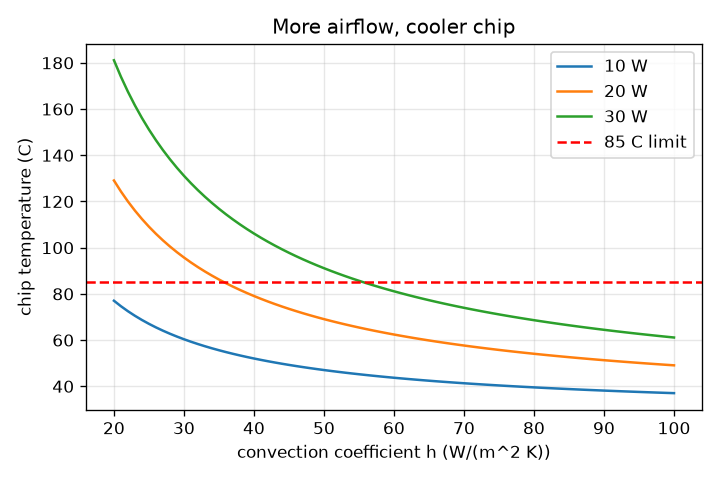
\includegraphics[width=0.85\linewidth]{figures/s02_chip_vs_airflow.png}\\\small Chip temperature against convection coefficient for 10, 20 and 30 W, with the 85 C limit.\end{center}

\subsection*{E. Worked example}
A 20 W chip sits on 0.2 mm of paste (k = 3 W/(m K)) and a 3 mm aluminium base (k = 200 W/(m K)), both over 4 cm\textasciicircum{}2. Air with h = 50 W/(m\textasciicircum{}2 K) cools 100 cm\textasciicircum{}2 of fins at 25 C. Find the chip temperature and the temperature at each interface.
\begin{enumerate}[nosep]
\item R\_paste = 0.0002 / (3 * 0.0004) = 0.1667 K/W.
\item R\_base = 0.003 / (200 * 0.0004) = 0.0375 K/W.
\item R\_air = 1 / (50 * 0.01) = 2.0000 K/W. R\_total = 0.1667 + 0.0375 + 2.0000 = 2.2042 K/W.
\item T\_chip = 25 + 20 * 2.2042 = 69.08 C.
\item Drops: paste 20 * 0.1667 = 3.33 K (chip 69.08 C to 65.75 C), base 20 * 0.0375 = 0.75 K (to 65.00 C), air 20 * 2.0 = 40 K (to 25 C).
\item Sanity check: the drops 3.33 + 0.75 + 40 = 44.08 K add up to 69.08 - 25.
\end{enumerate}
\textbf{Answer.} The chip is at 69.08 C; the fins are at 65.00 C. The air film takes 40 K of the 44 K total.

\subsection*{F. Questions}
\begin{enumerate}[nosep]
\item \textbf{Conceptual.} The thermal paste is only 0.2 mm thick and the base is 3 mm thick, yet the air film has far more resistance than either. Why?
\item \textbf{Numerical.} A 15 W chip sits on the same paste and a 4 mm copper base (k = 400), with h = 40 W/(m\textasciicircum{}2 K) on 100 cm\textasciicircum{}2 of fins. Find the chip temperature.
\item \textbf{Graph and simulation interpretation.} On the airflow graph for 10, 20 and 30 W, which of those chips stay below 85 C at h = 50 W/(m\textasciicircum{}2 K)? Roughly where does the 30 W curve cross 85 C?
\item \textbf{Design and optimisation challenge.} Design: a 30 W chip must stay at or below 85 C with the 3 mm aluminium base and h = 50. (a) Find the smallest h that works. (b) Would switching to a copper base (k = 400) be enough instead? (c) Suggest a design and a trade-off.
\end{enumerate}

\section{Session 3: A 2D heat solver, validated, and a laptop with two hot spots}

\subsection*{A. Real-world problem}
A laptop board has a CPU and a GPU that each create a small, intense hot spot. Metal under the board spreads the heat sideways and the fan carries it off the faces. Session 2 could only say 'heat flows through a layer'; it cannot say where the hot spots are or how they evolve in time. Can you write a small solver that predicts the temperature everywhere on the board, and how do you know it can be trusted? This is a simplified educational model, not a design tool for real products.

\subsection*{B. Concept and theory}
In a thin sheet, the temperature changes with time according to the diffusion (heat) equation: the rate of change of T equals the thermal diffusivity alpha times the sum of the second derivatives of T in x and in y. The second derivative measures how much a point differs from the average of its neighbours. On a grid of square cells of size dx, the explicit update moves each cell a fraction r = alpha dt / dx\textasciicircum{}2 of the way toward the average of its four neighbours. If r is larger than 1/4 a cell overshoots the average and the errors grow every step; so dt must not exceed dx\textasciicircum{}2 / (4 alpha). Heat sources add a term P / (rho c V) in K/s, and cooling of the two faces by air subtracts a term 2 h T / (rho c d). Validation means comparing against cases with exact answers: a steady wall (straight-line profile) and a Gaussian hot spot, whose exact solution in an unbounded sheet stays Gaussian with width squared s0\textasciicircum{}2 + 2 alpha t.

\begin{itemize}[nosep]
\item T: temperature rise above room temperature (K)
\item alpha: thermal diffusivity k / (rho c); aluminium about 82 mm\textasciicircum{}2/s (mm\textasciicircum{}2/s)
\item dx, dt: cell size and time step (mm, s)
\item r: stability number alpha dt / dx\textasciicircum{}2 (no unit)
\item A, s0: initial peak rise (60 K) and width (3 mm) of the Gaussian hot spot (K, mm)
\item P: chip power (W)
\item rho c: volumetric heat capacity of the sheet (aluminium 2.43e6) (J/(m\textasciicircum{}3 K))
\item d, h: sheet thickness and convection coefficient (mm, W/(m\textasciicircum{}2 K))
\end{itemize}

\begin{equation*}
\frac{\partial T}{\partial t}=\alpha\left(\frac{\partial^2 T}{\partial x^2}+\frac{\partial^2 T}{\partial y^2}\right)
\end{equation*}

\begin{equation*}
T^{n+1}_{i,j}=T^{n}_{i,j}+r\left(T_{i-1,j}+T_{i+1,j}+T_{i,j-1}+T_{i,j+1}-4T_{i,j}\right),\quad r=\frac{\alpha\,\Delta t}{\Delta x^2}\le\frac14
\end{equation*}

\begin{equation*}
T(x,y,t)=A\,\frac{s_0^2}{s_0^2+2\alpha t}\exp\!\left(-\frac{x^2+y^2}{2\,(s_0^2+2\alpha t)}\right)
\end{equation*}

\begin{equation*}
\frac{\partial T}{\partial t}=\alpha\nabla^2T+\frac{P}{\rho c\,V}-\frac{2h}{\rho c\,d}\,T
\end{equation*}

\begin{center}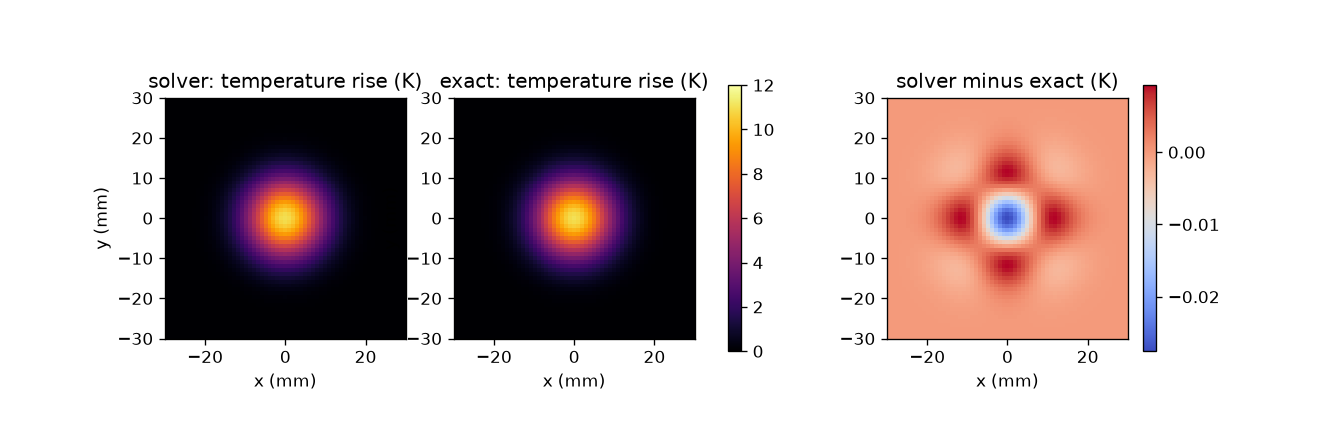
\includegraphics[width=0.85\linewidth]{figures/s03_gaussian_spreading.png}\\\small A Gaussian hot spot after 1 s: solver, exact solution and their difference.\end{center}

\subsection*{E. Worked example}
For a material with alpha = 20 mm\textasciicircum{}2/s on a grid with dx = 1 mm, find the largest stable time step, then find the peak temperature rise of the 60 K, 3 mm Gaussian hot spot after 1 s, from the exact formula, and compare with the solver at r = 0.2.
\begin{enumerate}[nosep]
\item dt\_max = dx\textasciicircum{}2 / (4 alpha) = 1 / (4 * 20) = 0.0125 s. With r = 0.2 we use dt = 0.2 * 1 / 20 = 0.01 s, so 100 steps reach 1 s.
\item Exact width: s0\textasciicircum{}2 + 2 alpha t = 9 + 2 * 20 * 1 = 49 mm\textasciicircum{}2.
\item Exact peak = 60 * 9 / 49 = 11.02 K (the hot spot has dropped from 60 K to about 11 K by spreading).
\item The solver gives 10.99 K, a difference of 0.03 K (0.2 percent).
\item Sanity check: heat is conserved by the insulated edges, so as the peak falls the hot spot must become wider; the width went from 3 mm to 7 mm (sqrt 49).
\end{enumerate}
\textbf{Answer.} dt\_max = 0.0125 s; exact peak 11.02 K after 1 s; the solver gives 10.99 K.

\subsection*{F. Questions}
\begin{enumerate}[nosep]
\item \textbf{Conceptual.} Why does the explicit scheme blow up when dt is too large, even though each step only moves a cell toward the average of its neighbours?
\item \textbf{Numerical.} Aluminium has alpha = 82.3 mm\textasciicircum{}2/s. Find the largest stable time step for dx = 0.5 mm. What happens to dt\_max if you halve dx again?
\item \textbf{Graph and simulation interpretation.} In the convergence plot the largest errors are 0.449, 0.110, 0.0275 and 0.0069 K for dx = 4, 2, 1 and 0.5 mm. By what factor does the error shrink each time dx is halved? Predict the error at dx = 0.25 mm, then check with \texttt{max\_error(0.25)}.
\item \textbf{Design and optimisation challenge.} Design: the CPU (12 W) and GPU (8 W) must stay at most 85 C in 25 C air (a rise of at most 60 K) with h = 40 W/(m\textasciicircum{}2 K). The 100 mm x 60 mm aluminium spreader sheet (2.7 g per cm\textasciicircum{}3) may not weigh more than 20 g. Using the printed table, choose a thickness and justify it.
\end{enumerate}

\section{Real-world mini-project}
\textbf{Thermal budget for a laptop with two hot spots.} A laptop has a 12 W CPU and an 8 W GPU on a 100 mm x 60 mm board backed by an aluminium spreader sheet. A fan gives h = 40 W/(m\textasciicircum{}2 K). The chips must stay at most 80 C when the room is 25 C, so the peak temperature rise must be at most 55 K. Use \texttt{peak\_rise} and \texttt{board\_run} from Session 3 to choose the sheet thickness. Aluminium weighs 2.7 g per cm\textasciicircum{}3 and the sheet may weigh at most 25 g. This is a simplified educational model, not a design tool.

\section{The path ahead}
\begin{enumerate}[nosep]
\item \textbf{Session 4: An implicit solver with no step limit.} A second solver that runs the Gaussian test with steps many times larger than the explicit limit.
\item \textbf{Session 5: A heat pipe between the chips and the edge.} A board model with a high-conductance strip connecting the CPU to the board edge.
\item \textbf{Session 6: Go 3D: a stack of chip, board and spreader.} The same validation in three dimensions with layers of different materials.
\item \textbf{Session 7: Reproduce the Target: bare board against spreader.} A transient simulation of two chips switching on and off and an animated heat map.
\item \textbf{Session 8: Find the hot spots from a few sensors.} A script that recovers CPU and GPU power from three noisy sensor readings.
\end{enumerate}

\section{Answers and hints}

\subsection*{Session 1}
\begin{enumerate}[nosep]
\item \textbf{Conceptual.} Hint: Think about what the profile depends on, and what Q depends on. Solution: Both have exactly the same straight-line profile: the drop per millimetre is (T\_hot - T\_cold) / L, which does not contain k. Copper carries far more heat, because Q is proportional to k (400 against about 1 W/(m K), so roughly 400 times more). The conductivity decides how much heat flows, not how the temperature is shaped.
\item \textbf{Numerical.} Hint: Convert 0.5 mm and 1 cm\textasciicircum{}2 to metres first. Q = k A dT / L. Solution: Q = 5 * 0.0001 * 20 / 0.0005 = 20 W. Units: W/(m K) times m\textasciicircum{}2 times K divided by m gives W. Sanity check: compared with the worked example (15 W) the pad is half as thick, which would double the flow, but the temperature drop is smaller (20 K against 30 K), which cuts it by a third: 15 * 2 * 2/3 = 20 W.
\item \textbf{Graph and simulation interpretation.} Hint: Use T = 80 - 40 x / L. Remember the 2 mm slab ends at 2 mm. Solution: L = 2 mm: 80 - 40 * 2 / 2 = 40 C (the cold face). L = 5 mm: 80 - 16 = 64 C. L = 10 mm: 80 - 8 = 72 C. The slopes are 20, 8 and 4 C per mm: the thicker the slab, the more gently the temperature falls, because the same 40 C difference is spread over more distance.
\item \textbf{Design and optimisation challenge.} Hint: Rearrange the law: L = k A dT / Q gives the largest allowed thickness. Solution: Largest thickness: L = 5 * 0.0001 * 30 / 12 = 0.00125 m = 1.25 mm. So any thickness from 0.3 mm to 1.25 mm works. A choice of 0.5 mm carries 5 * 0.0001 * 30 / 0.0005 = 30 W, a comfortable margin. Trade-off: thinner pads carry more heat but are harder to make and to press flat on an uneven chip; thicker pads are forgiving but run out of margin at 1.25 mm.
\end{enumerate}

\subsection*{Session 2}
\begin{enumerate}[nosep]
\item \textbf{Conceptual.} Hint: Compare L/(kA) with 1/(hA): which has a small number in the denominator? Solution: R = 1/(hA) uses h of only 50 W/(m\textasciicircum{}2 K) on 0.01 m\textasciicircum{}2, a product of 0.5 W/K, while the base has k A / L = 200 * 0.0004 / 0.003 = 27 W/K. Moving air is a very weak heat road compared with solid metal, even though the film has no thickness in the model. That is why the air side usually dominates and why designers add fins (bigger A) and fans (bigger h).
\item \textbf{Numerical.} Hint: Compute the three resistances, add them, then T = 25 + P R\_total. Solution: R\_paste = 0.1667 K/W. R\_base = 0.004 / (400 * 0.0004) = 0.025 K/W. R\_air = 1 / (40 * 0.01) = 2.5 K/W. R\_total = 2.6917 K/W. T\_chip = 25 + 15 * 2.6917 = 65.4 C. Sanity check: R\_total is slightly larger than R\_air alone (2.5), as it must be.
\item \textbf{Graph and simulation interpretation.} Hint: Evaluate T = 25 + P * 2.2042 at the three powers and read the 30 W crossing from the graph. Solution: At h = 50: 10 W gives 47.0 C, 20 W gives 69.1 C and 30 W gives 91.1 C. So 10 and 20 W stay below 85 C and 30 W does not. The 30 W curve crosses 85 C near h = 56 W/(m\textasciicircum{}2 K) (the design formula gives 55.7).
\item \textbf{Design and optimisation challenge.} Hint: For (a) use the h\_min formula. For (b) recompute R\_base and T\_chip at h = 50. Solution: (a) Allowed total R = (85 - 25) / 30 = 2.0 K/W, so R\_air \textless{}= 2.0 - 0.1667 - 0.0375 = 1.7958 K/W and h \textgreater{}= 1 / (1.7958 * 0.01) = 55.7 W/(m\textasciicircum{}2 K). (b) With copper R\_base = 0.01875 and R\_total = 2.1854 K/W, so T = 25 + 30 * 2.1854 = 90.6 C (aluminium gives 91.1 C): still above 85 C, copper only gains 0.6 K. (c) Raise h to about 60 (a faster fan), or add fins to raise A\_fins; or throttle the chip power to 27 W (max power of the original cooler at 85 C is 27.2 W). Trade-offs: a faster fan costs noise and battery; more fins cost size and weight; throttling costs performance. Keep a safety margin because the model is simplified.
\end{enumerate}

\subsection*{Session 3}
\begin{enumerate}[nosep]
\item \textbf{Conceptual.} Hint: What happens if a cell moves MORE than the whole way to the average (r larger than 1/4 in 2D)? Solution: With r above 1/4 the new value overshoots the neighbour average, so the cell ends on the far side of it. The checkerboard error pattern is then multiplied by \textbar{}1 - 8 r\textbar{} each step, which is bigger than 1 when r is above 1/4 (1.4 at r = 0.30), so errors grow geometrically instead of fading. A finer grid makes the limit tighter because dt\_max goes with dx\textasciicircum{}2.
\item \textbf{Numerical.} Hint: dt\_max = dx\textasciicircum{}2 / (4 alpha). Solution: dt\_max = 0.25 / (4 * 82.3) = 0.00076 s (0.76 ms). Halving dx makes dx\textasciicircum{}2 four times smaller, so dt\_max becomes 0.00019 s. In 2D that means four times more cells and four times more steps: sixteen times the work. Sanity check: a finer grid always needs a smaller step.
\item \textbf{Graph and simulation interpretation.} Hint: Divide each error by the next one. Solution: The ratios are 4.08, 4.00 and 4.00: the error falls by 4 each time dx is halved, so the method is second order (error proportional to dx\textasciicircum{}2). At dx = 0.25 mm the lesson's own run (\texttt{max\_error(0.25)}, r = 0.2) gives 0.0017 K, a factor 4.0 below 0.0069 K, as expected for a second-order method.
\item \textbf{Design and optimisation challenge.} Hint: The sheet is 60 cm\textasciicircum{}2, so mass = 60 * d(cm) * 2.7 g. Compare the peak rises in the table. Solution: The sheet is 60 cm\textasciicircum{}2, so mass = 60 * d(cm) * 2.7 g: 0.5 mm gives 8.1 g, 1.0 mm gives 16.2 g and 2.0 mm gives 32.4 g. At h = 40 the peak rises are 76.3 K (0.5 mm), 59.7 K (1.0 mm) and 50.9 K (2.0 mm). Only 1.0 mm meets both the 60 K limit and the 20 g limit, but it passes by only 0.3 K, which is too thin a margin for a simplified model. A better design raises h as well: at h = 80 the 1.0 mm sheet gives 38.2 K. Trade-off: a faster fan costs noise and battery; a thicker sheet costs weight.
\end{enumerate}

\section{How to join}
Read \texttt{CONTRIBUTING.md} in the repository, then pick an issue labelled \texttt{good first issue}. Repository: \url{https://github.com/KrunalPanchal1995/openheatspread}

\end{document}
